% Chapter 2

\chapter{Haptic Search Experiment} % Main chapter title

\label{Haptic Search Experiment} % For referencing the chapter elsewhere, use \ref{Haptic Search Experiment} 

%----------------------------------------------------------------------------------------
%In diesem Kapitel wird der Versuch, die benutzte Hardware , %und das komplette Setting von der Aufnahme beschrieben

%----------------------------------------------------------------------------------------
\section{Haptic Search Experiment}
\subsection{Experimental Setup}
The Modular Haptic Stimuli Board (MHSB) makes up the core part of the experiment. It is a setting with two wooden frames that hold stimuli objects. These objects are 3 x 3 cm big wooden blocks, which have a primitive three-dimensional shape on top of it or are just plane. The whole set consists of 360 blocks with 55 different shapes.\\
The first wooden frame can fit 25 objects and is used for learning a target object whereas the second frame has a capacity of 100 objects and is used for searching target objects. The stimuli are statically installed in the frames and not manipulable to allow a focus on just the search task itself (see Figure \ref{MHSBBOARDS}).\\
\\
For this experiment, a subset of stimuli was chosen, consisting of 5 different shapes and plane ones (see Figure \ref{Stimuli}). The target consists of one object and is placed central in the small frame with the rest of the space consisting of plane stimuli. The big frame contains the rest of this subset, where each shape exist 4 to 5 times, including the target. The objects were distributed mostly equally and kept the same rotation throughout the experiment. Only the distribution and the target were changed with each trial.\\

\begin{figure}[H]
	\centering
	\begin{minipage}{0.49\textwidth}
		\centering
		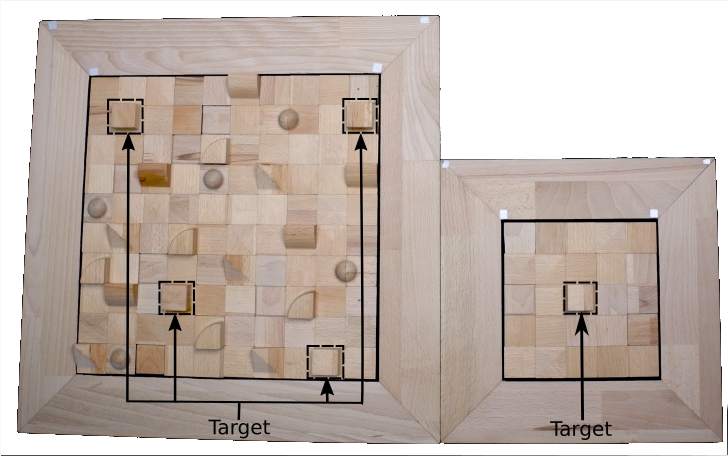
\includegraphics[width=\textwidth]{MHSB_cut}
		\captionsetup{width=0.9\textwidth}
		\caption{MHSB: on the right side for learning, on the left for search task. The arrows point to the target instances.}
		\label{MHSBBOARDS}
	\end{minipage}
	\begin{minipage}{0.49\textwidth}
		\centering
		\includegraphics[width=0.85\textwidth]{Stimuli}
		\captionsetup{width=0.9\textwidth}
		\caption{Stimuli objects used in the MHSB. From left: Wave, Sphere, Quarter, Box, Pyramid}
		\label{Stimuli}
	\end{minipage}
\end{figure}


\subsection{Execution}  
For this experiment, 7 participants were invited and asked to solve a haptic search task while being blindfolded. The participants were 23 to 28 years old and included both genders. All participants were right-handed and have never seen the stimuli objects, so that during the task they never knew how the set of objects looked like and their perception was purely based on the haptic features.\\
Each participant performed on maximal 5 trials, where after each trial, the target was exchanged and the distribution of the stimuli on the big frame was changed. Before the beginning, there were 2 rehearsals to accustom the subjects to the setting. No participant had the same target twice or more and the task was done with just the right hand, while wearing a glove to record relevant data (See \ref{Hardware}).\\
\\
For the procedure, each participant was given a description of the task (See Appendix \ref{AppendixA}). The task consisted of two parts. \\
The first task was to explore the target object on the small frame and remembering it just by its haptic features. When collected enough information about the target stimulus, the subject should proceed to the big frame and search for the learned target. The only goal in this part was to remember the approximate position of the target and not saying that it was found or pointing at it, so the recorded data would not contain pauses or pointing postures.\\
It was not necessary to find every target shape in the big frame, just as many as one could. The time was limited to 30 seconds to guarantee that the focus lies only on the salient features. An acoustic signal by the examiner determined the start- and endpoint of the experiment.\\
The second part of the experiment was to figure out if the subjects found the target object between the non-target objects, called distractors, and how well they could remember the approximate position on the frame. Again an acoustic signal determined start and end of the trial. For the second part, the subjects had just 10 seconds left to find the targets and point on them. The short period of time was set to prevent the subjects from exploring too much of the frame and focusing only on the smallest set of haptic features that were sufficient enough to differentiate between target and distractor.\\

%----------------------------------------------------------------------------------------
\section{Hardware} \label{Hardware}
In this section the used hardware will be described as well as the overall setting that was used to record the data for the experiment.\\
There will be first a brief description of the glove that was used to capture tactile relevant and hand posture data followed by a description of the Vicon system to capture position data in a three-dimensional environment. At the end the implementation of the hardware into the experimental setting is explained.

\subsection{Glove}
A detailed explanation of the underlying technical properties and its implementation into the glove can be found in the work of Bianchi et. al. \cite{Glove}.\\
\\
To record data for this experiment, a device was needed that would be able to capture the most relevant patterns underlying a haptic search task. These so called exploratory features (EPs) describe the behavior of the hand during the exploration \cite{EPs}. Furthermore a device for recording the tactile properties was needed.\\
The multi-modal sensing glove combines both of these features. On the bottom side of the glove 64 tactile cells are mounted, covering hand palm and fingers. These fabric-based sensors record local pressures with a frequency of 150 Hz. The top side consists of 18 bending sensors, used to capture the joint angles representing the hand pose with a frequency of 50 Hz.
 
\subsection{Vicon}
For capturing the position of the hand and the MHSB, the Vicon system was used \cite{Vicon}. It records motion data with a frequency of 200 Hz, using retroreflective markers that are tracked by infrared cameras.\\
Also included is a Basler camera, generating a top-down view for the experiment.

\subsection{Setting}
To record motion data from the subjects hand, 17 reflective markers has been placed on an extra glove that the participant wears atop of the multi-modal one. The markers were placed in a position as shown in Figure \ref{Glove_markers} to guarantee a good reconstruction of the finger and hand movements.\\
The most time-consuming part was to find a setting of the Vicon cameras that would capture the reflective markers continuously, making sure to minimize the occurrence of gaps. The result is shown in Figure \ref{Setting} There were 14 Vicon cameras placed in a semicircle around the MHSB. The Basler camera was placed directly above the frames. As an addition, there were 2 cameras placed on the left and right side to record also the side-view of the experiment.\\
The glove was connected via USB and serial-port to a nearby computer. A second computer controlled the Vicon system. To simultanetly start the recording, a synchronising tool called MSS was used (See \ref{recording}).

\begin{figure}[H]
	\centering
	\begin{minipage}{0.49\textwidth}
		\centering
		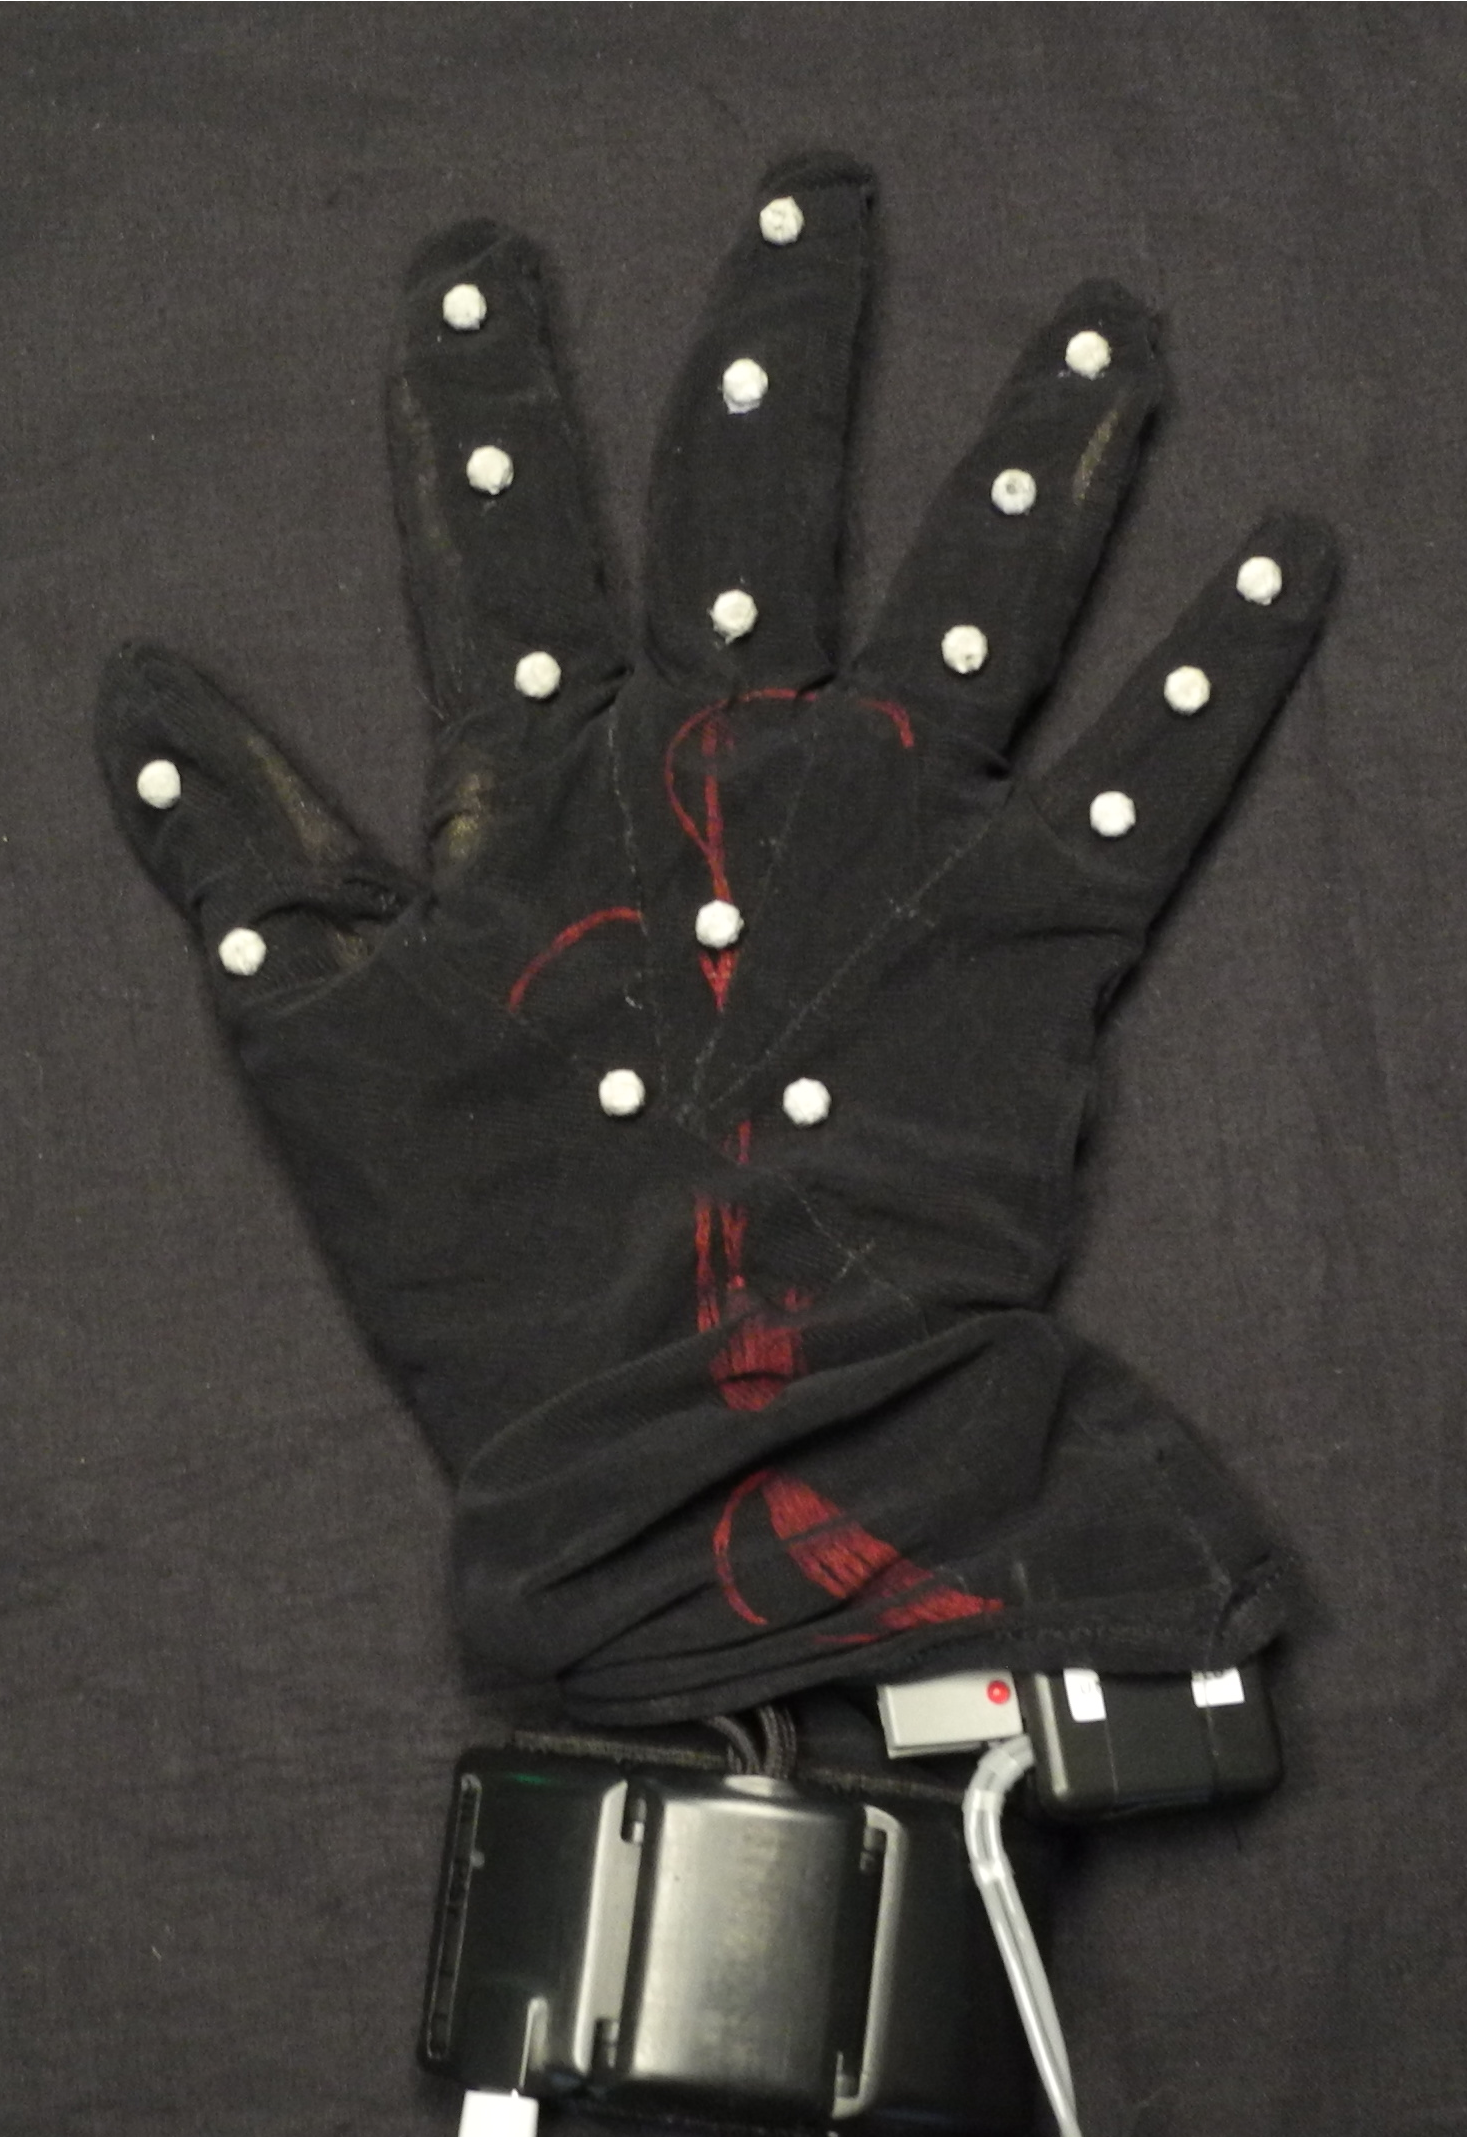
\includegraphics[width=0.55\textwidth]{glove_markers}
		\captionsetup{width=0.9\textwidth}
		\caption{Glove with 17 retroreflective markers for tracking the hand movement with Vicon}
		\label{Glove_markers}
	\end{minipage}
	\begin{minipage}{0.49\textwidth}
		\centering
		\includegraphics[width=\textwidth]{Setting}
		\captionsetup{width=0.9\textwidth}
		\caption{Experimental setting with MHSB, glove and Vicon cameras}
		\label{Setting}
	\end{minipage}
\end{figure}
 